\documentclass[11pt,class=report,crop=false]{standalone}
\usepackage[screen]{../python}


\begin{document}


%====================================================================
\chapitre{Tri -- Complexité}
%====================================================================

\index{tri}
\index{complexite@complexité}

\objectifs{Ordonner les éléments d'une liste est une activité essentielle en informatique. Par exemple une fois qu'une liste est triée, il est très facile de chercher 
si elle contient tel ou tel élément. Par définition un algorithme renvoie toujours le résultat attendu, mais certains algorithmes sont plus rapides que d'autres ! Cette efficacité est mesurée par la notion de complexité.}

\bigskip

Ce chapitre commence par de la théorie : tout d'abord des rappels sur les suites et l'explication de la notation \og{}grand O\fg{}. Ensuite on aborde la notion de complexité qui mesure la performance d'un algorithme. Ceux qui veulent coder peuvent directement s'attaquer aux différents algorithmes de tris présentés. Le bilan est fait dans la dernière activité : comparer les complexités des différents algorithmes de tris.

\bigskip

%%%%%%%%%%%%%%%%%%%%%%%%%%%%%%%%%%%%%%%%%%%%%%%%%%%%%%%%%%%%%%%%
%%%%%%%%%%%%%%%%%%%%%%%%%%%%%%%%%%%%%%%%%%%%%%%%%%%%%%%%%%%%%%%%

\begin{cours}[Notation \og{}grand O\fg{}]
\index{grand O}
On souhaite comparer deux suites, ou plus exactement leur ordre de grandeur. Par exemple les suites $(n^2)_{n\in\Nn}$ et $(3n^2)_{n\in\Nn}$ ont le même ordre de grandeur, mais sont beaucoup plus petites que la suite $(\frac12 e^n)_{n\in\Nn}$. 

\textbf{Notation \og{}grand O\fg{}.}
\begin{itemize}
	\item On considère $(u_n)_{n\in\Nn}$ et $(v_n)_{n\in\Nn}$ deux suites de termes strictement positifs.
	\item On dit que $(u_n)$ est un \defi{grand O} de $(v_n)$ si la suite $\left(\frac{u_n}{v_n}\right)$ est bornée.
    \item Autrement dit il existe une constante réelle $k>0$ telle que pour tout $n\in \Nn$:
$$u_n \le k v_n.$$
    \item \emph{Notation.} On note alors $u_n = O(v_n)$. Il s'agit de la lettre \og{}O\fg{} (pour Ordre de grandeur) et pas du chiffre zéro.
\end{itemize}

\emph{Exemples} 
\begin{itemize}
	\item Soient $u_n = 3n+1$ et $v_n = 2n-1$. Comme $\frac{u_n}{v_n} \to \frac{3}{2}$ lorsque $n\to+\infty$ alors la suite $\left(\frac{u_n}{v_n}\right)$ est bornée donc $u_n = O(v_n)$.
	
	\item $u_n = 2n^2$ et $v_n = e^n$. Comme $\frac{u_n}{v_n} \to 0$ alors la suite $\left(\frac{u_n}{v_n}\right)$ est bornée donc $u_n = O(v_n)$. 
	
	\item $u_n = \sqrt{n}$ et $v_n = \ln(n)$. Comme $\frac{u_n}{v_n} \to +\infty$ lorsque $n\to+\infty$ alors la suite $\left(\frac{u_n}{v_n}\right)$ n'est pas bornée.  $(u_n)$ n'est pas un grand O de $(v_n)$.  Par contre dans l'autre sens, on a bien $v_n = O(u_n)$.
	
	\item $u_n \in O(n)$ signifie qu'il existe $k>0$ tel que $u_n \le kn$ (pour tout $n\in\Nn$).
	
	\item $u_n \in O(1)$ signifie que la suite $(u_n)$ est bornée.
		
\end{itemize}

\bigskip

\textbf{Suites de référence.}
\index{suite}
\index{logarithme}
\index{exponentielle}

On va de préférence comparer une suite $(u_n)$ avec des suites de référence. Voici les suites de référence choisies :
$$\underbrace{\ln(n)}_{\text{croissance logarithmique}} \quad \underbrace{n \quad  n^2 \quad n^3 \quad  \cdots}_{\text{croissance polynomiale}} \quad \underbrace{e^n}_{\text{croissance exponentielle}}$$

\begin{itemize}
	\item Les suites sont écrites en respectant l'ordre des O : on a $\ln(n) = O(n)$, $n=O(n^2)$, $n^2=O(n^3)$, \ldots, $n^3 = O(e^n)$.
	
	\item On pourrait intercaler d'autres suites, par exemple $\ln(n) = O(\sqrt{n})$ et $\sqrt{n} = O(n)$.
	Ou encore $n\ln(n) = O(n^2)$.
	
	\item Il est important de savoir visualiser ces suites (voir le graphique de l'activité 1).
\end{itemize}

\end{cours}


%%%%%%%%%%%%%%%%%%%%%%%%%%%%%%%%%%%%%%%%%%%%%%%%%%%%%%%%%%%%%%%%
% Activité 1 - Notation \og{}grand O\fg{}
%%%%%%%%%%%%%%%%%%%%%%%%%%%%%%%%%%%%%%%%%%%%%%%%%%%%%%%%%%%%%%%%

\begin{activite}[Notation \og{}grand O\fg{}]
   
\objectifs{Objectifs : comparer des suites avec la notation  \og{}grand O\fg{}.}
 
\begin{enumerate}
	
  \item Considère les suites définies par 
  $$u_n = 1000 n^2 \qquad \text{ et } \qquad v_n = 0.001 \exp(n)$$
  
  Calcule les premiers termes de chaque suite. Penses-tu que $u_n =O(v_n)$ ou bien $v_n = O(u_n)$ ?
	
	
  \item Visualise les termes de différentes suites, comme sur le graphique ci-dessous
  où tu retrouves les termes des suites $\ln(n)$, $\sqrt{n}$, $n$, $n^2$, $e^n$.

 \begin{center}
 	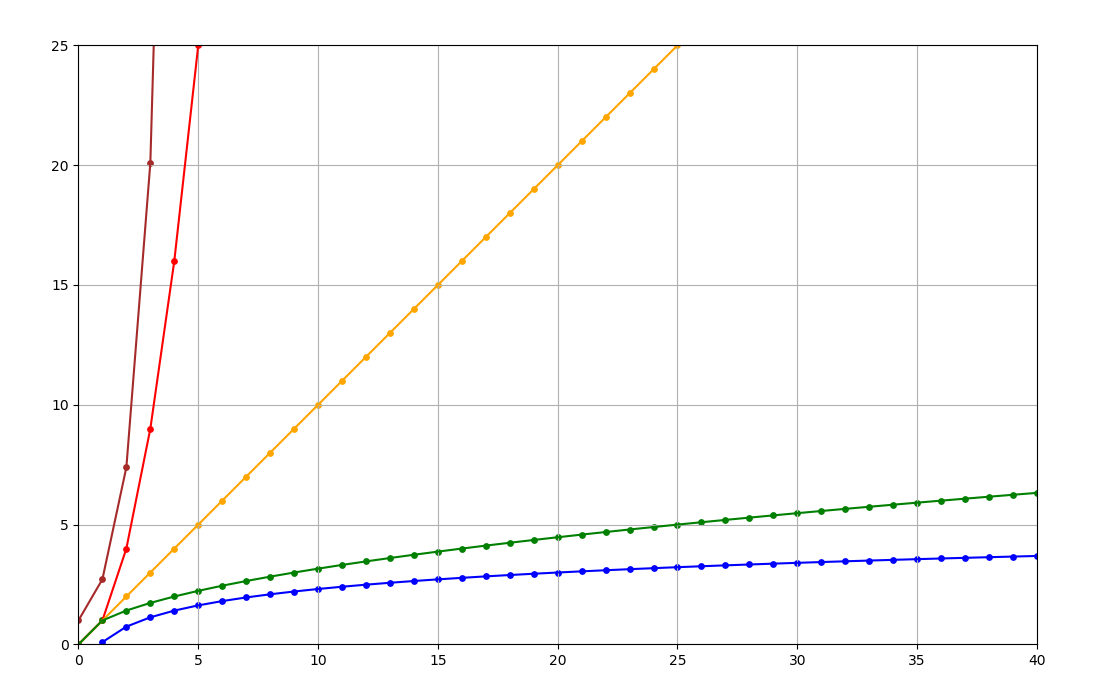
\includegraphics[scale=\myscale,scale=0.3]{ecran-grandO}
 	
 	\emph{Les suites  $\ln(n)$, $\sqrt{n}$, $n$, $n^2$, $e^n$.}
 \end{center} 

  \item Programme une fonction \ci{est_grand_O(u,v)} qui renvoie \og{}Vrai\fg{} si la suite $(u_n)$ est expérimentalement un grand O de $(v_n)$.
  On dira que $(u_n)$ est expérimentalement un grand O de $(v_n)$ si 
  $$u_n \le k v_n$$
  pour $n \in [10,1000]$ et $k=10$. (Bien sûr le choix de ces constantes est arbitraire.)
  
  A-t-on expérimentalement $n^2 = O(2^n)$ ? Et $n = O(\sqrt{n})$ ?
  
  Tu peux définir une suite \ci{u} comme une fonction :
  \mycenterline{\ci{def u(n): return n**2}}  
  ou bien   
  \mycenterline{\ci{u = lambda n: n**2}}  
  Dans les deux cas on obtient le terme $u_n$ par la commande \ci{u(n)}.
  
\end{enumerate}

\end{activite}


%%%%%%%%%%%%%%%%%%%%%%%%%%%%%%%%%%%%%%%%%%%%%%%%%%%%%%%%%%%%%%%%
%%%%%%%%%%%%%%%%%%%%%%%%%%%%%%%%%%%%%%%%%%%%%%%%%%%%%%%%%%%%%%%%

\begin{cours}[Complexité d'un algorithme]
On mesure l'efficacité d'un algorithme à l'aide de la complexité. 

\begin{itemize}
	\item Les deux principales caractéristiques qui font qu'un algorithme est bon ou mauvais sont la rapidité d'exécution et l'utilisation de la mémoire. Nous nous limiterons ici à étudier la vitesse d'exécution. 
	
	\item Comment mesurer la vitesse ? Une durée (en secondes) dépend de chaque ordinateur et n'est pas un indicateur universel. 
	
	\item Aussi nous définissons de manière informelle la complexité : la \defi{complexité} d'un algorithme est le nombre d'opérations élémentaires exécutées.
	
	\item Ce que l'on appelle \og{}opération élémentaire\fg{} peut varier selon le contexte : pour un calcul cela peut être le nombre de multiplications, pour un tri le nombre de comparaisons\ldots
	
	\item La complexité $C_n$ dépend de la taille $n$ des données en entrée (par exemple le nombre de chiffres d'un entier ou bien la longueur de la liste). On obtient ainsi une suite $(C_n)$.
	
	\item Le bons algorithmes ont des complexités polynomiales qui sont en $O(n)$ (linéaire), ou en $O(n^2)$ (quadratique) ou bien en $O(n^k)$, $k\in\Nn^*$ (polynomiale). Les mauvais algorithmes ont des complexités exponentielles, en $O(e^n)$ par exemple.
\end{itemize}

\bigskip

\textbf{Multiplication de deux entiers.}

On souhaite multiplier deux entiers $a$ et $b$ de $n$ chiffres.
Il y a plusieurs méthodes, on les compare en comptant le nombre d'opérations élémentaires : ici des multiplications de petits nombres (entiers à $1$ ou $2$ chiffres).

\begin{center}
	\begin{tabular}{|c|c|}\hline
		Algorithme  & Ordre de la complexité \\ \hline\hline
		Multiplication d'école & $O(n^2)$ \\ \hline
		Multiplication de Karatsuba & $O(n^{\log_2(3)}) \simeq O(n^{1.53})$  \\ \hline
		Transformée de Fourier rapide & $O(n\cdot \ln(n) \cdot \ln(\ln(n))$  \\\hline
	\end{tabular}
\end{center}  

Voici des exemples d'ordre de grandeur de la complexité pour différentes valeurs de $n$.
\begin{center}
	\begin{tabular}{|c|c|c|c|}\hline
		Algorithme  & $n=10$ & $n=100$ & $n=1000$  \\ \hline\hline
		Multiplication d'école & $100$ & $10\,000$ & $1\,000\,000$ \\ \hline
		Multiplication de Karatsuba & $38$ & $1478$ &  $56\,870$ \\ \hline
		Transformée de Fourier rapide & $19$ & $703$ & $13\,350$   \\\hline
	\end{tabular}
\end{center} 

Plus l'entier $n$ est grand, plus un bon algorithme prend l'avantage.

\bigskip

\textbf{Recherche dans une liste.}

La recherche d'un élément dans une liste non triée nécessite de tester chaque élément de la liste.
Si la liste est de longueur $n$ alors il faut $O(n)$ tests.
Par contre si la liste est ordonnée alors il existe des algorithmes beaucoup plus efficaces : par exemple la recherche par dichotomie (voir le chapitre \og{}Le mot le plus long\fg{}).


\begin{center}
	\begin{tabular}{|c|c|}\hline
		Algorithme  & Ordre de la complexité \\ \hline\hline
		\'Elément par élément (liste non triée) & $O(n)$ \\ \hline
		Dichotomie (liste triée) & $O(\log_2(n))$  \\ \hline
	\end{tabular}
\end{center}

Voici des exemples d'ordre de grandeur de la complexité pour différentes valeurs de $n$.
\begin{center}
	\begin{tabular}{|c|c|c|c|}\hline
		Algorithme  & $n=1000 =10^3$ & $n=10^6$ & $n=10^9$  \\ \hline\hline
		\'Elément par élément & $10^3$ & $10^6$ & $10^9$ \\ \hline
		Dichotomie & $10$ & $20$ &  $30$ \\ \hline
	\end{tabular}
\end{center} 

\bigskip

\textbf{Problème du voyageur de commerce.}

On se donne $n$ villes et les distances entre ces villes. Il s'agit de trouver le plus court chemin qui visite toutes les villes en revenant à la ville de départ. Il n'y pas d'algorithme connu qui soit efficace pour obtenir la meilleure solution. Un des meilleurs algorithmes a pour complexité $O(n^2  2^n)$.
Voici des exemples d'ordre de grandeur de la complexité pour différentes valeurs de $n$.
\begin{center}
	\begin{tabular}{|c|c|c|c|}\hline
		Algorithme  & $n=10$ & $n=100$ & $n=1000$  \\ \hline\hline
		Voyageur de commerce & $10^5$ & $10^{34}$ & $10^{307}$ \\ \hline

	\end{tabular}
\end{center} 

On voit que cet algorithme est inutilisable sauf pour de petites valeurs de $n$.

 	
\end{cours}


%%%%%%%%%%%%%%%%%%%%%%%%%%%%%%%%%%%%%%%%%%%%%%%%%%%%%%%%%%%%%%%%
%%%%%%%%%%%%%%%%%%%%%%%%%%%%%%%%%%%%%%%%%%%%%%%%%%%%%%%%%%%%%%%%

\begin{cours}[Le tri avec \Python]
\sauteligne
\begin{itemize}
	
	\item  La commande \Python{} pour ordonner une liste est \ci{sorted()}.\index{sort@\ci{sort/sorted}}
	Par exemple avec \ci{liste = [5, 6, 1, 8, 10]}, la commande \ci{sorted(liste)} renvoie la nouvelle liste \ci{[1, 5, 6, 8, 10]} dans laquelle les éléments sont ordonnés du plus petit au plus grand.
	
	Cela fonctionne aussi avec des chaînes de caractères, pour	
	\mycenterline{\ci{liste = ['BATEAU', 'ABRIS', 'ARBRE', 'BARBE']}}	
	 alors \ci{sorted(liste)} renvoie \ci{['ABRIS', 'ARBRE', 'BARBE', 'BATEAU']} ordonnée selon l'ordre alphabétique.
	
	\item Variante. La méthode \ci{liste.sort()} ne renvoie rien, mais après utilisation de cette méthode, \ci{liste} est ordonnée (on parle de modification en place).
	
	\item Pour obtenir un tri dans l'ordre inverse, utilise la commande \ci{sorted(liste, reverse = True)}.
	
	\item  Variante. \ci{list(reversed(sorted(liste)))}.
\end{itemize}
\end{cours}

%%%%%%%%%%%%%%%%%%%%%%%%%%%%%%%%%%%%%%%%%%%%%%%%%%%%%%%%%%%%%%%%
%%%%%%%%%%%%%%%%%%%%%%%%%%%%%%%%%%%%%%%%%%%%%%%%%%%%%%%%%%%%%%%%

\begin{cours}[Double affectation avec \Python]
\index{double affectation}	
\Python{} permet les affectations multiples, ce qui permet d'échanger facilement le contenu de deux variables.
	\begin{itemize}
		\item \textbf{Affectation multiple.} 		
		\mycenterline{\ci{a, b = 3, 4}}
		
		Maintenant \ci{a} vaut $3$ et \ci{b} vaut $4$.
		
		\item \textbf{\'Echange de valeurs.}		
		\mycenterline{\ci{a, b = b, a}}		
		Maintenant \ci{a} vaut l'ancien contenu de \ci{b} donc vaut $4$ et \ci{b} vaut l'ancien contenu de \ci{a} donc $3$.
		
		\item \textbf{\'Echange à la main.} Pour échanger deux valeurs sans utiliser la double affectation, il faut introduire une variable temporaire :
\begin{center} 
\begin{lstlisting}		
temp = a
a = b
b = temp			
\end{lstlisting}
\end{center}
\end{itemize}
\end{cours}
	


%%%%%%%%%%%%%%%%%%%%%%%%%%%%%%%%%%%%%%%%%%%%%%%%%%%%%%%%%%%%%%%%
% Activité 2 - Tri par sélection
%%%%%%%%%%%%%%%%%%%%%%%%%%%%%%%%%%%%%%%%%%%%%%%%%%%%%%%%%%%%%%%%

\begin{activite}[Tri par sélection]
	\index{tri!selection@sélection}
	
	\objectifs{Objectifs : programmer le \og{}tri par sélection\fg{} qui est un algorithme très simple.}
	
	Il s'agit d'ordonner les éléments d'une liste du plus petit au plus grand.
	On note $n$ la longueur de la liste. Les éléments sont donc indexés de $0$ à $n-1$.
	
	\begin{algorithme}
	\sauteligne 	
		\begin{itemize}
			\item 
			\begin{itemize}
				\item Entrée : une liste de longueur $n$.				
				\item Sortie : la liste ordonnée.				
			\end{itemize}
			
			\item Pour $i$ variant de $0$ à $n-1$ :
			\begin{itemize}

				\item \emph{Recherche du plus petit élément après le rang $i$ :}
				
				\item \ci{rg_min} $\leftarrow i$
				
				\item pour $j$ allant de $i+1$ à $n-1$ :\\
				\indentation si \ci{liste[j]} < 	\ci{liste[rg_min]} faire  \ci{rg_min} $\leftarrow j$.
											
				\item \emph{\'Echange.} \'Echanger l'élément de rang $i$ avec l'élément de rang \ci{rg_min}.
					
			\end{itemize}			
						
			\item Renvoyer la liste.			
		\end{itemize}
	\end{algorithme}   
	
	\bigskip
	
	\textbf{Explications.}
 L'algorithme est très simple : on cherche le plus petit élément de la liste et on le place en tête.
 Le premier élément est donc à sa place. On recommence avec le reste de la liste : on cherche le plus petit élément que l'on positionne en deuxième place\ldots
 
 \myfigure{0.5}{
 	\tikzinput{fig_tri_1}
 }
 	\bigskip
	
	\textbf{Travail à faire.} Programme cet algorithme en une fonction \ci{tri_selection(liste)}.
	
		
	\emph{Indications.} La fonction ne doit pas modifier la liste passée en paramètre. Pour éviter les désagréments :
	\begin{itemize}
		\item commence par faire une copie de ta liste:		
		\mycenterline{\ci{cliste = list(liste)}}		
		\item ne travaille qu'avec \ci{cliste}, que tu peux modifier à volonté,
		\item renvoie \ci{cliste}.
	\end{itemize}

    \emph{Commentaires.}
	Le principal avantage de cet algorithme est sa simplicité. Sinon il est de complexité $O(n^2)$ ce qui en fait un algorithme de tri lent réservé pour les petites listes.
    
	
\end{activite}


%%%%%%%%%%%%%%%%%%%%%%%%%%%%%%%%%%%%%%%%%%%%%%%%%%%%%%%%%%%%%%%%
% Activité 3 - Tri par insertion
%%%%%%%%%%%%%%%%%%%%%%%%%%%%%%%%%%%%%%%%%%%%%%%%%%%%%%%%%%%%%%%%

\begin{activite}[Tri par insertion]
\index{tri!insertion}

\objectifs{Objectifs : programmer le \og{}tri par insertion\fg{} qui est un algorithme très simple.}

Le tri par insertion est assez naturel : c'est le tri que tu utilises par exemple pour trier un jeu de cartes. 
Tu prends les deux premières cartes, tu les ordonnes. Tu prends la troisième carte, tu la places au bon endroit pour obtenir trois cartes bien ordonnées. Tu prends une quatrième carte que tu places au bon endroit pour obtenir quatre cartes bien ordonnées\ldots

	\begin{algorithme}
	\sauteligne 	
	\begin{itemize}
		\item 
		\begin{itemize}
			\item Entrée : une liste de longueur $n$.				
			\item Sortie : la liste ordonnée.				
		\end{itemize}
		
		\item Pour $i$ variant de $1$ à $n-1$ :
		\begin{itemize} 
			\item \ci{el} $\leftarrow$ \ci{liste[i]} \quad  \emph{(on mémorise l'élément pivot de rang $i$)}
			\item \emph{On décale vers la droite tous les éléments de rang $i-1$ à $0$ qui sont plus grands que le pivot :}  
			\item $j \leftarrow i$
			\item Tant que $(j>0)$ et $($\ci{liste[j-1]} $>$ \ci{el}$)$:
			\begin{itemize}
				\item \ci{liste[j]} $\leftarrow$ \ci{liste[j-1]}
				\item $j \leftarrow j-1$
			\end{itemize}
			\item \ci{liste[j]} $\leftarrow$ \ci{el} \quad  \emph{(on replace l'élément pivot dans le trou créé par le décalage)}
		\end{itemize}			
		
		\item Renvoyer la liste.			
	\end{itemize}
\end{algorithme} 

	\bigskip

\textbf{Explications.}
L'algorithme est assez simple : on regarde les deux premiers éléments, s'ils sont dans le mauvais sens on les échange (les deux premiers éléments sont maintenant bien ordonnés entre eux).
On regarde ensuite les trois premiers éléments, on insère le troisième élément à la bonne place parmi ces trois éléments (qui sont maintenant bien ordonnés entre eux). On recommence avec les quatre premiers éléments : on insère le quatrième élément à la bonne place parmi ces quatre éléments\ldots

Le dernier élément du groupe considéré est appelé pivot,  pour l'insérer on décale d'un rang vers la droite tous les élément situés avant lui qui sont plus grands. On obtient donc un trou qui est la place du pivot.

\myfigure{0.5}{
	\tikzinput{fig_tri_2}
}

\bigskip

\textbf{Travail à faire.} Programme cet algorithme en une fonction \ci{tri_insertion(liste)}.

\bigskip

    \emph{Commentaires.}
    C'est un bon algorithme dans la catégorie des algorithmes de tri lents ! Il est de complexité $O(n^2)$, mais sur une liste déjà un peu ordonnée il est efficace. Il est un peu meilleur que le tri par sélection. Il permet aussi d'ordonner des éléments en \og{}temps réels\fg{} : on peut commencer à trier le début de la liste sans connaître la fin. 

\end{activite}




%%%%%%%%%%%%%%%%%%%%%%%%%%%%%%%%%%%%%%%%%%%%%%%%%%%%%%%%%%%%%%%%
% Activité 4 - Tri à bulles
%%%%%%%%%%%%%%%%%%%%%%%%%%%%%%%%%%%%%%%%%%%%%%%%%%%%%%%%%%%%%%%%

\begin{activite}[Tri à bulles]
	
\index{tri!a bulles@à bulles}
	
	\objectifs{Objectifs : programmer le \og{}tri à bulles\fg{}.}
	
	Le tri à bulles est très simple à programmer : il s'agit d'échanger deux termes consécutifs s'ils ne sont pas dans le bon ordre. Le nom vient de l'analogie avec les bulles d'eau qui remontent à la surface comme ici les éléments qui viennent se positionner à leur place.
	
		\begin{algorithme}
		\sauteligne 
		
		\begin{itemize}
			\item 
			\begin{itemize}
				\item Entrée : une liste de longueur $n$.			
				\item Sortie : la liste ordonnée.				
			\end{itemize}
			
			\item Pour $i$ allant de $n-1$ à $0$ :\\
				\indentation Pour $j$ allant de $0$ à $i-1$ :\\
				\indentation\indentation Si \ci{liste[j+1]} $<$ \ci{liste[j]} alors :\\
				\indentation\indentation\indentation échanger \ci{liste[j]} et \ci{liste[j+1]}.
			
			
			\item Renvoyer la liste.
			
		\end{itemize}
	\end{algorithme} 

	\bigskip

\textbf{Explications.}
L'algorithme est très simple : on compare deux éléments consécutifs et on les échange s'ils sont dans le mauvais ordre.
On continue avec les couples suivants jusqu'à la fin de la liste. Au bout du premier passage le dernier élément est définitivement à sa place.
On recommence en partant du début avec un second passage, maintenant les deux derniers éléments sont à leur place. 

\myfigure{0.5}{
	\tikzinput{fig_tri_3}
}

\bigskip

\textbf{Travail à faire.} Programme cet algorithme en une fonction \ci{tri_a_bulles(liste)}.

\bigskip

\emph{Commentaires.} Le tri à bulles est très simple à programmer, cependant il fait aussi partie des algorithmes de 
tri lents car sa complexité est en $O(n^2)$.
	
\end{activite}



%%%%%%%%%%%%%%%%%%%%%%%%%%%%%%%%%%%%%%%%%%%%%%%%%%%%%%%%%%%%%%%%
% Activité 5 - Tri fusion
%%%%%%%%%%%%%%%%%%%%%%%%%%%%%%%%%%%%%%%%%%%%%%%%%%%%%%%%%%%%%%%%

\begin{activite}[Tri fusion]
	
	\index{tri!fusion}
	
	\objectifs{Objectifs : programmer un tri beaucoup plus efficace : le \og{}tri fusion\fg{}. Par contre sa programmation est plus compliquée car l'algorithme est récursif.}
	
	Le tri fusion est un tri rapide. Il est basé sur le principe de \og{}diviser pour régner\fg{} ce qui fait que sa programmation naturelle se fait
	par une fonction récursive. Le principe est simple : on divise la liste en deux parties ; on trie la liste de gauche (par un appel récursif) ; on trie la liste de droite (par un autre appel récursif) ; ensuite il faut fusionner ces deux listes en intercalant les termes.
	
	
	Ce tri se programme à l'aide de deux fonctions : une fonction principale \ci{tri_fusion(liste)} qui trie la liste. Cette fonction nécessite la fonction secondaire \ci{fusion(liste_gauche,liste_droite)} qui fusionne deux listes triées en une seule. 
	
	\bigskip 
	
	On commence par la fonction principale qui est une fonction récursive.
	\begin{algorithme}
	\sauteligne 
	
	\begin{itemize}
		\item 
		\begin{itemize}
			\item Entête : \ci{tri_fusion(liste)} 
			\item Entrée : une liste de longueur $n$.			
			\item Sortie : la liste ordonnée.		
			\item Action : fusion récursive.		
		\end{itemize}
		
		\item \emph{Cas terminal.} Si la liste est de longueur $0$ ou $1$, renvoyer la liste telle quelle.
		
		\item \emph{Cas général.} 
		
		\item Calculer \ci{liste_g = tri_fusion(liste[:n//2])}. On prend les éléments de gauche (de rang $< n//2$) et on les trie par un appel récursif.
		
		\item Calculer \ci{liste_d = tri_fusion(liste[n//2:])}. On prend les éléments de droite (de rang $\ge n//2$) et on les trie par un appel récursif.
		
		\item Renvoyer la liste \ci{fusion(liste_g,liste_d)}.
		
	\end{itemize}
\end{algorithme} 

	La fonction précédente nécessite la fonction définie par l'algorithme suivant :
		\begin{algorithme}
		\sauteligne 
		
		\begin{itemize}
			\item 
			\begin{itemize}
				\item Entête : \ci{fusion(liste_g,liste_d)} 
				\item Entrée : deux listes ordonnées : \ci{liste_g} de longueur $n$ et \ci{liste_d} de longueur $m$.			
				\item Sortie : une liste fusionnée et ordonnée.				
			\end{itemize}
			
			\item 
			\begin{itemize}
				\item Un indice $i$, initialisé à $0$, indexe la première liste, 
				\item un indice $j$, initialisé à $0$, indexe la seconde liste,
				\item une liste \ci{liste_fus} est initialisée à la liste vide.
			\end{itemize} 
			
			\item \emph{Fusion principale.}
			
			Tant que $(i < n)$ et $(j < m)$, faire:
			\begin{itemize}
				\item si \ci{liste_g[i]} $<$ \ci{liste_d[j]} ajouter  \ci{liste_g[i]} à \ci{liste_fus} et incrémenter $i$,
				\item sinon  ajouter  \ci{liste_d[j]} à \ci{liste_fus} et incrémenter $j$.
			\end{itemize} 	
			\item \emph{S'il reste des termes.}
			\begin{itemize}
			  \item Tant que $i < n$, ajouter  \ci{liste_g[i]} à \ci{liste_fus} et incrémenter $i$.
			  \item Tant que $j < m$, ajouter  \ci{liste_d[j]} à \ci{liste_fus} et incrémenter $j$.	
			\end{itemize} 			
			
			\item Renvoyer \ci{liste_fus}.
			
		\end{itemize}
	\end{algorithme} 
	
	
%	\begin{algorithme}
%	\sauteligne 
%	
%	\begin{itemize}
%		\item 
%		\begin{itemize}
%			\item Entête : \ci{fusion(liste_g,liste_d)} 
%			\item Entrée : deux listes ordonnées.			
%			\item Sortie : une liste fusionnée et ordonnée.		
%			\item Action : fonction récursive.		
%		\end{itemize}
%		
%		\item \emph{Cas terminaux.} Si une liste est vide, renvoyer l'autre.
%		
%		\item \emph{Cas général.}
%		
%		\item Si \ci{liste_g[0]} $\le$ \ci{liste_d[0]} alors :
%		\indentation renvoyer la liste \ci{[liste_g[0]] + fusion(liste_g[1:],liste_d)}
%		\item sinon renvoyer liste \ci{[liste_d[0]] + fusion(liste_g,liste_d[1:])}
%		
%	\end{itemize}
%\end{algorithme} 



\bigskip

\textbf{Explications.}
La seconde fonction \ci{fusion()} regroupe deux listes ordonnées en une seule liste ordonnée.
La fonction \ci{tri_fusion(liste)} est très simple, comme nous l'avons expliqué précédemment : la liste est découpée en une partie droite et une partie gauche. Grâce à deux appels récursifs chacune de ces sous-parties est triée. Il ne reste plus qu'à fusionner ces deux listes. 

\myfigure{0.5}{
	\tikzinput{fig_tri_4}
}

Bien sûr, comme toute fonction récursive, c'est assez difficile d'appréhender l'enchaînement complet des instructions.



Pourquoi cet algorithme est-il plus performant que les précédents ? Ce n'est pas facile à expliquer ! Le point-clé se passe lors la fusion : quand on fusionne deux listes ordonnées de longueur $n$ on effectue des comparaisons \ci{liste_g[i]} $<$ \ci{liste_d[j]}, mais on ne compare pas tous les éléments entre eux (ce qui donnerait $n^2$ comparaisons) mais seulement pour quelques couples $(i,j)$ ce qui donne $2n$ comparaisons.

\myfigure{0.4}{
	\tikzinput{fig_tri_5}
	\qquad\qquad
	\tikzinput{fig_tri_6}	
}


\bigskip

\textbf{Travail à faire.} Programme ces algorithmes en deux fonctions \ci{fusion(liste_g,liste_d)} et \ci{tri_fusion(liste)}.

\bigskip

\emph{Commentaires.} Le tri fusion est un tri rapide : sa complexité est $O(n\ln(n))$ ce qui est beaucoup mieux que les algorithmes précédents et est asymptotiquement optimal.
Il est conceptuellement simple à comprendre et à programmer si on connaît la récursivité.
	
\end{activite}


%%%%%%%%%%%%%%%%%%%%%%%%%%%%%%%%%%%%%%%%%%%%%%%%%%%%%%%%%%%%%%%%
% Activité 6 - Tri
%%%%%%%%%%%%%%%%%%%%%%%%%%%%%%%%%%%%%%%%%%%%%%%%%%%%%%%%%%%%%%%%

\begin{activite}[Complexité des algorithmes de tri]
	
	\objectifs{Objectifs : comparer expérimentalement les complexités des algorithmes de tri.}
	
	Pour les quatre algorithmes de tri que tu as programmés, modifie tes fonctions afin qu'elles renvoient en plus de la liste triée le nombre de comparaisons effectuées entre deux éléments de la liste. Chaque test du type \og{}\ci{liste[i]} $<$ \ci{liste[j]}\fg{} compte pour une comparaison.
	
	\bigskip
	
	\begin{itemize}
		\item Pour les trois premiers algorithmes, c'est assez facile ; pour le dernier c'est plus compliqué (voir ci-dessous).
		\item Compare le nombre de comparaisons effectuées : 
		\begin{itemize}
			\item quand la liste est une liste d'éléments tirés au hasard ; 
			\item quand la liste est déjà triée ;
			\item quand la liste est déjà triée mais en sens inverse.
		\end{itemize}
	\item On note $n$ la longueur de la liste. Compare la complexité avec $n^2$ (ou mieux $n^2/2$) pour les algorithmes lents et $n \ln(n)$ (ou mieux $n\log_2(n)$) pour l'algorithme de tri fusion.
	\end{itemize}

	\bigskip
	
	\emph{Indications pour le tri fusion.}
	Il faut commencer par modifier la fonction \ci{fusion()} en une fonction \ci{fusion_complexite()} qui renvoie en plus de la liste, le nombre de comparaisons effectuées lors de cette étape.
	Il faut ensuite modifier la fonction \ci{tri_fusion()} en une fonction \ci{tri_fusion_complexite()} qui renvoie en plus le nombre de comparaisons. Pour cela il faut compter le nombre de comparaisons venant du tri fusion de la partie gauche de la liste, le nombre de comparaisons venant du tri fusion de la partie droite de la liste, et enfin le nombre de comparaisons venant de la fusion. Il faut finalement renvoyer la somme de ces trois nombres.
	
\end{activite}

\bigskip

\objectifs{Une jolie activité consiste à visualiser pas à pas le tri d'une liste pour chaque algorithme. Voir les pages \emph{Wikipédia} pour un tel exemple d'animation.}

\end{document}
